\section*{Results}
\label{Results}


Using a 2-way ANOVA, a significant assessor effect (p<0.01) has been found on the dark-light attribute, which means that the assessors disagrees about how light/dark the speakers are.
\begin{figure}[H]
\centering
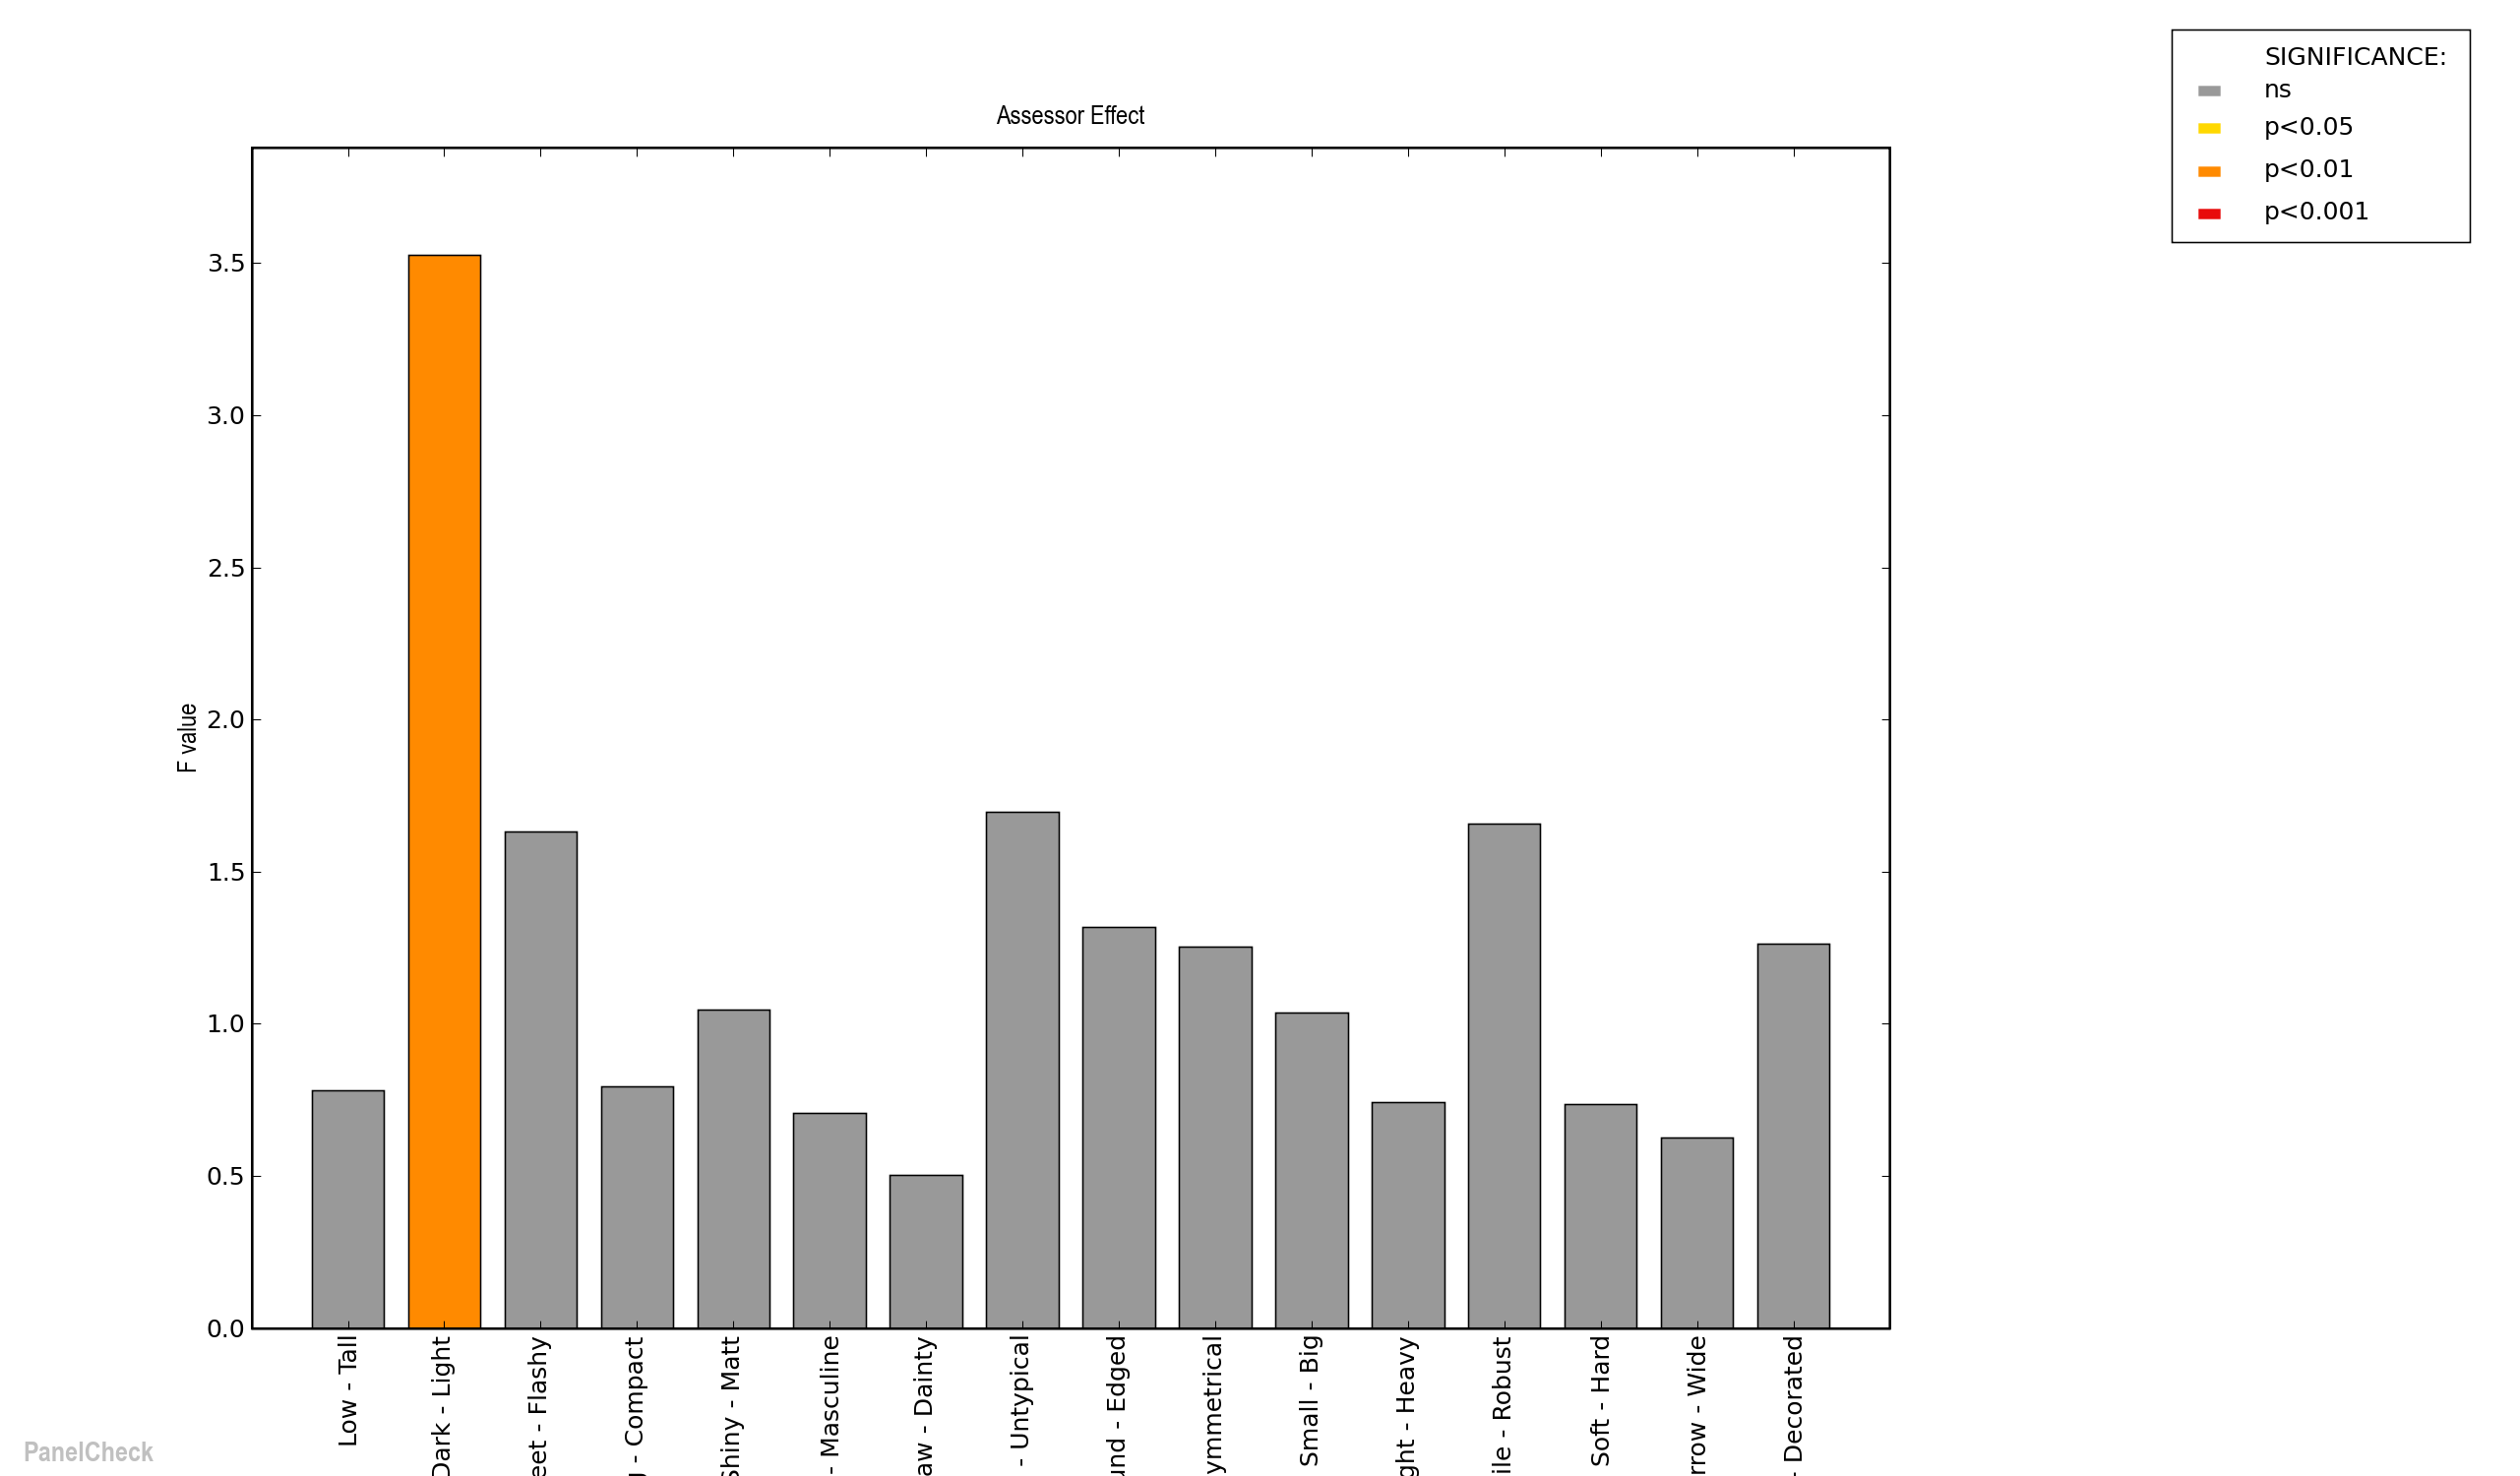
\includegraphics[width = 0.8\textwidth]{Figure/AssessorEffect.png} 
\caption{}
\label{fig:AssessorEffect}
\end{figure}
Regarding the product effect on ratings, all attributes are rated significant different at at least p<0.01, except for symmetrical-assymetrical. That means that the speaker model has an influence on the ratings of all the attributes, except for symmetry, which is unaffected of which speaker model is rated.
\begin{figure}[H]
\centering
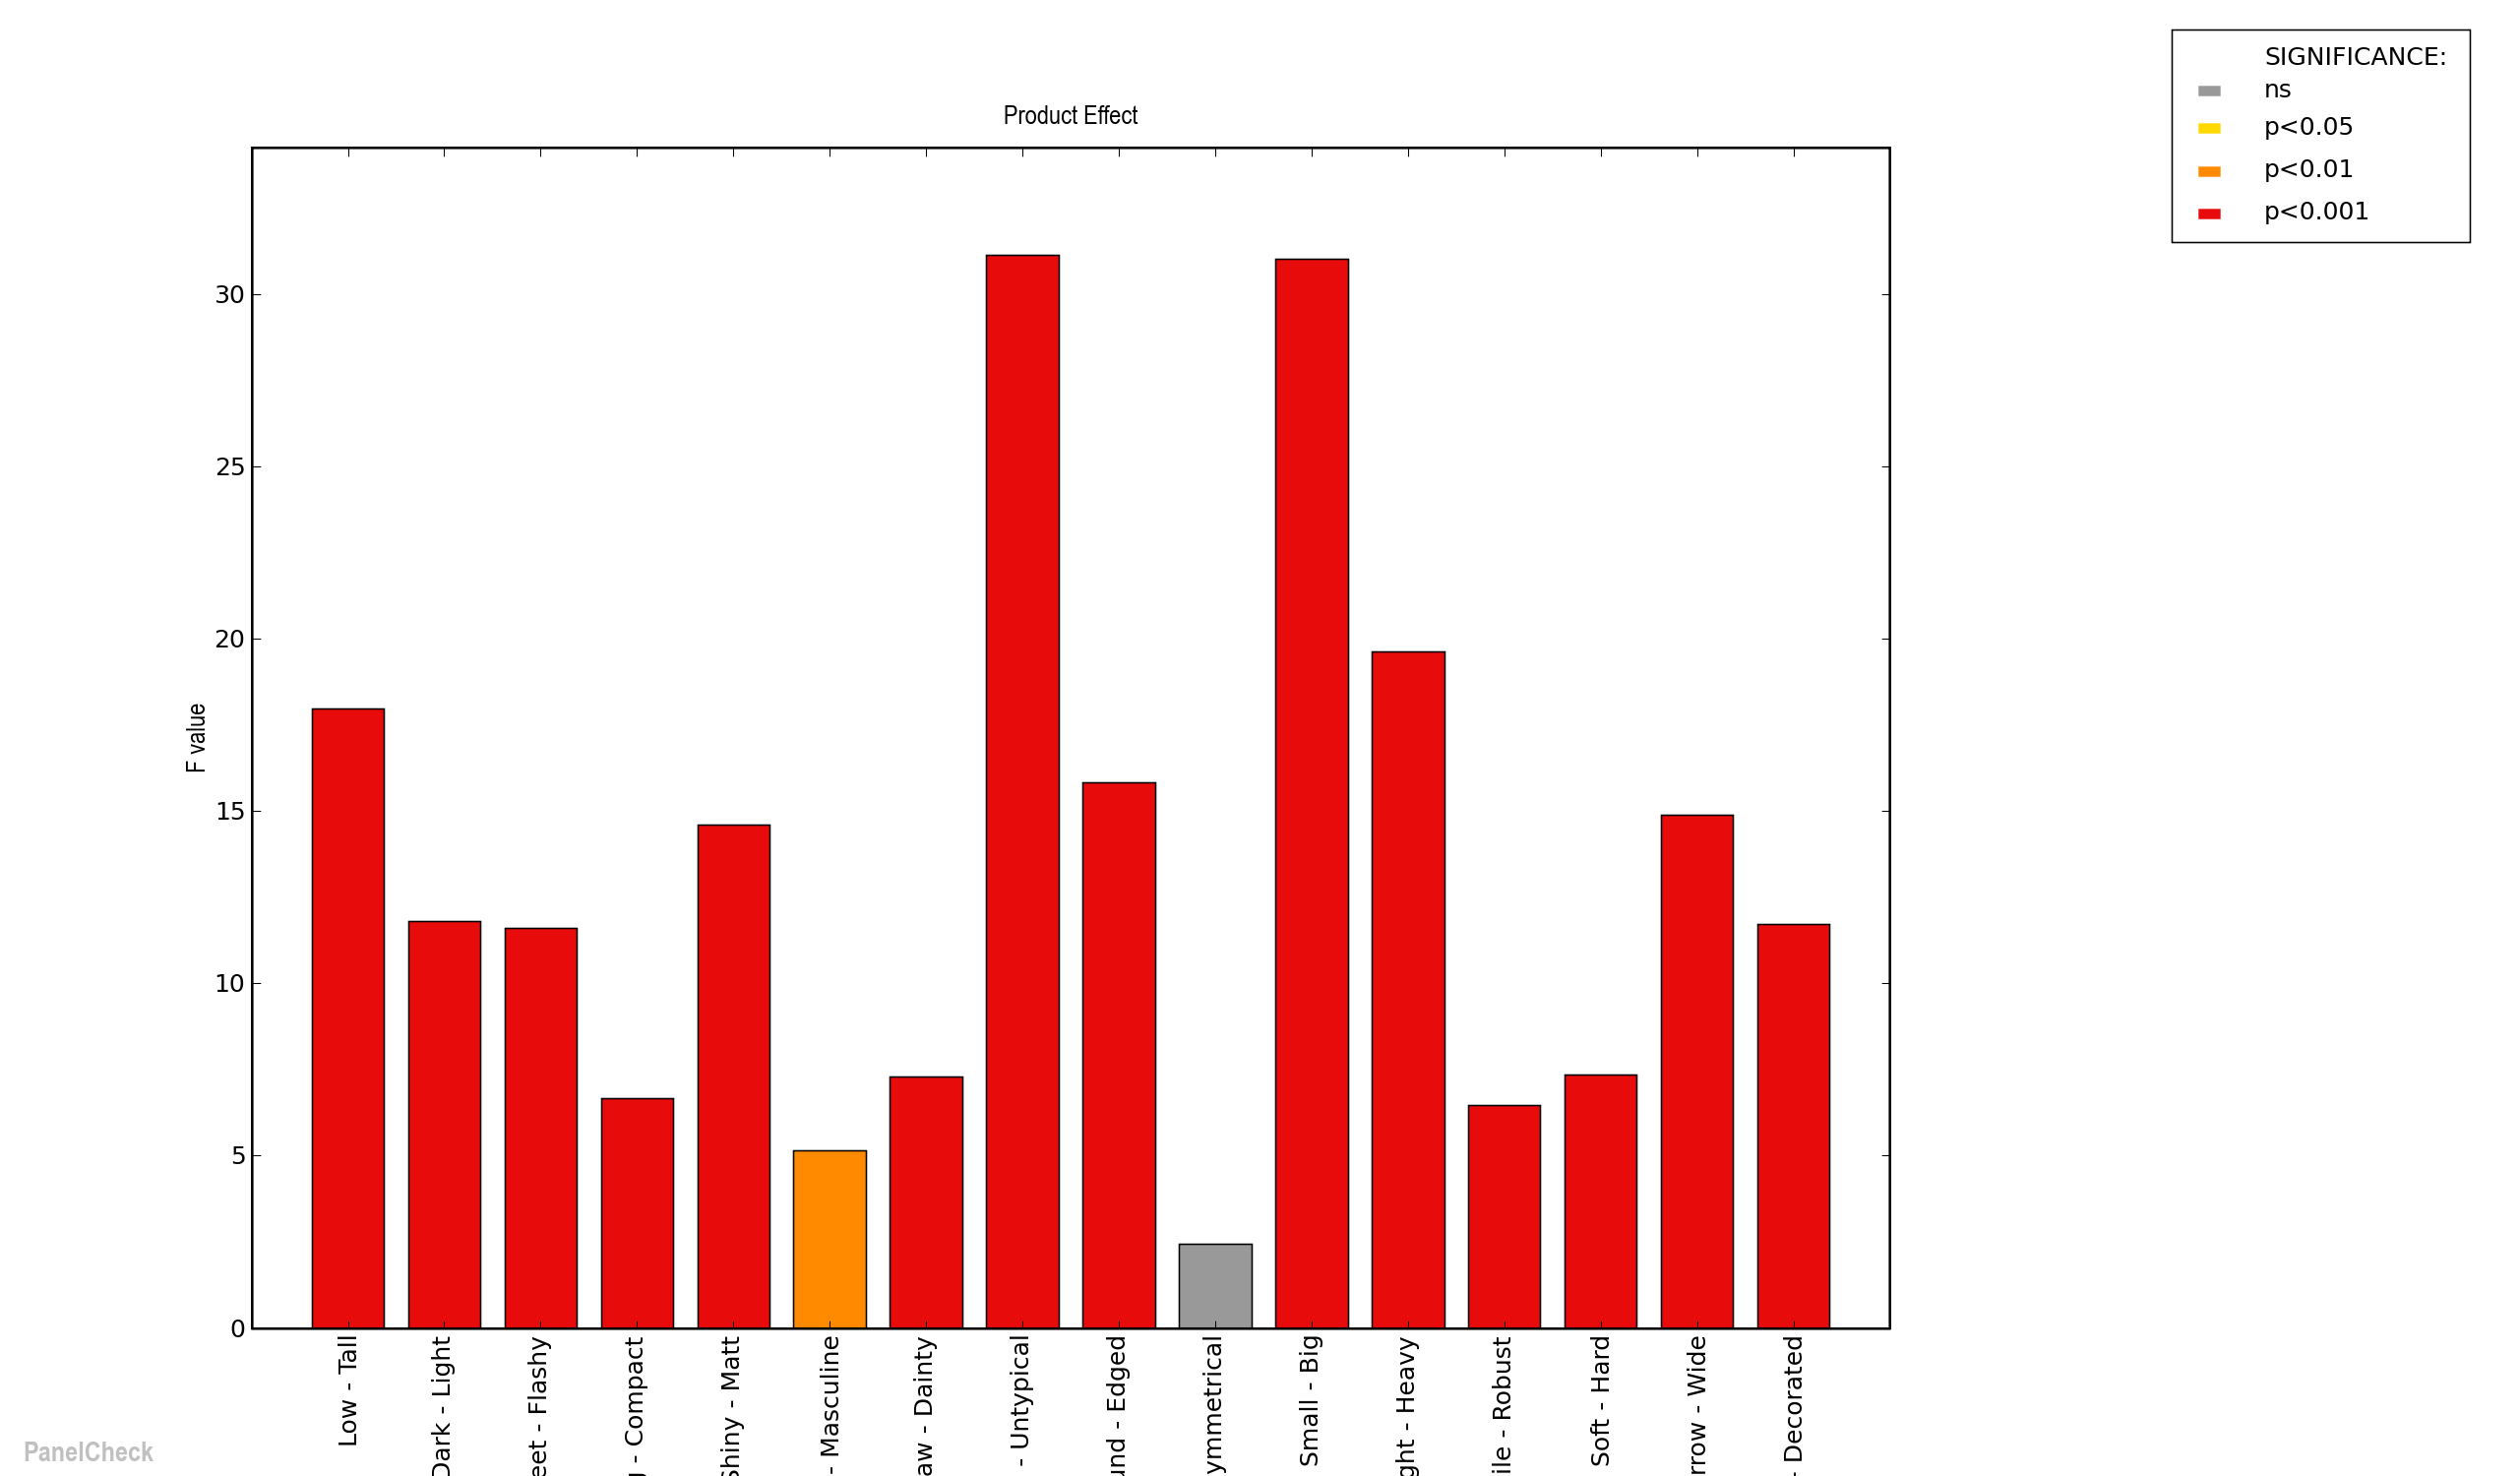
\includegraphics[width = 0.8\textwidth]{Figure/ProductEffect.png} 
\caption{ProductEffect}
\label{fig:ProductEffect}
\end{figure}

This can be confirmed by looking at the means and standard deviations for the different attributes. For example, in \autoref{fig:AttributeImportance}, the symmetry attribute has a very little standard deviation, which means that it is fairly unaffected by speaker model, compared to some of the other attributes. This means that the attribute is unimportant for the rating of the speakers.

\begin{figure}[H]
\centering
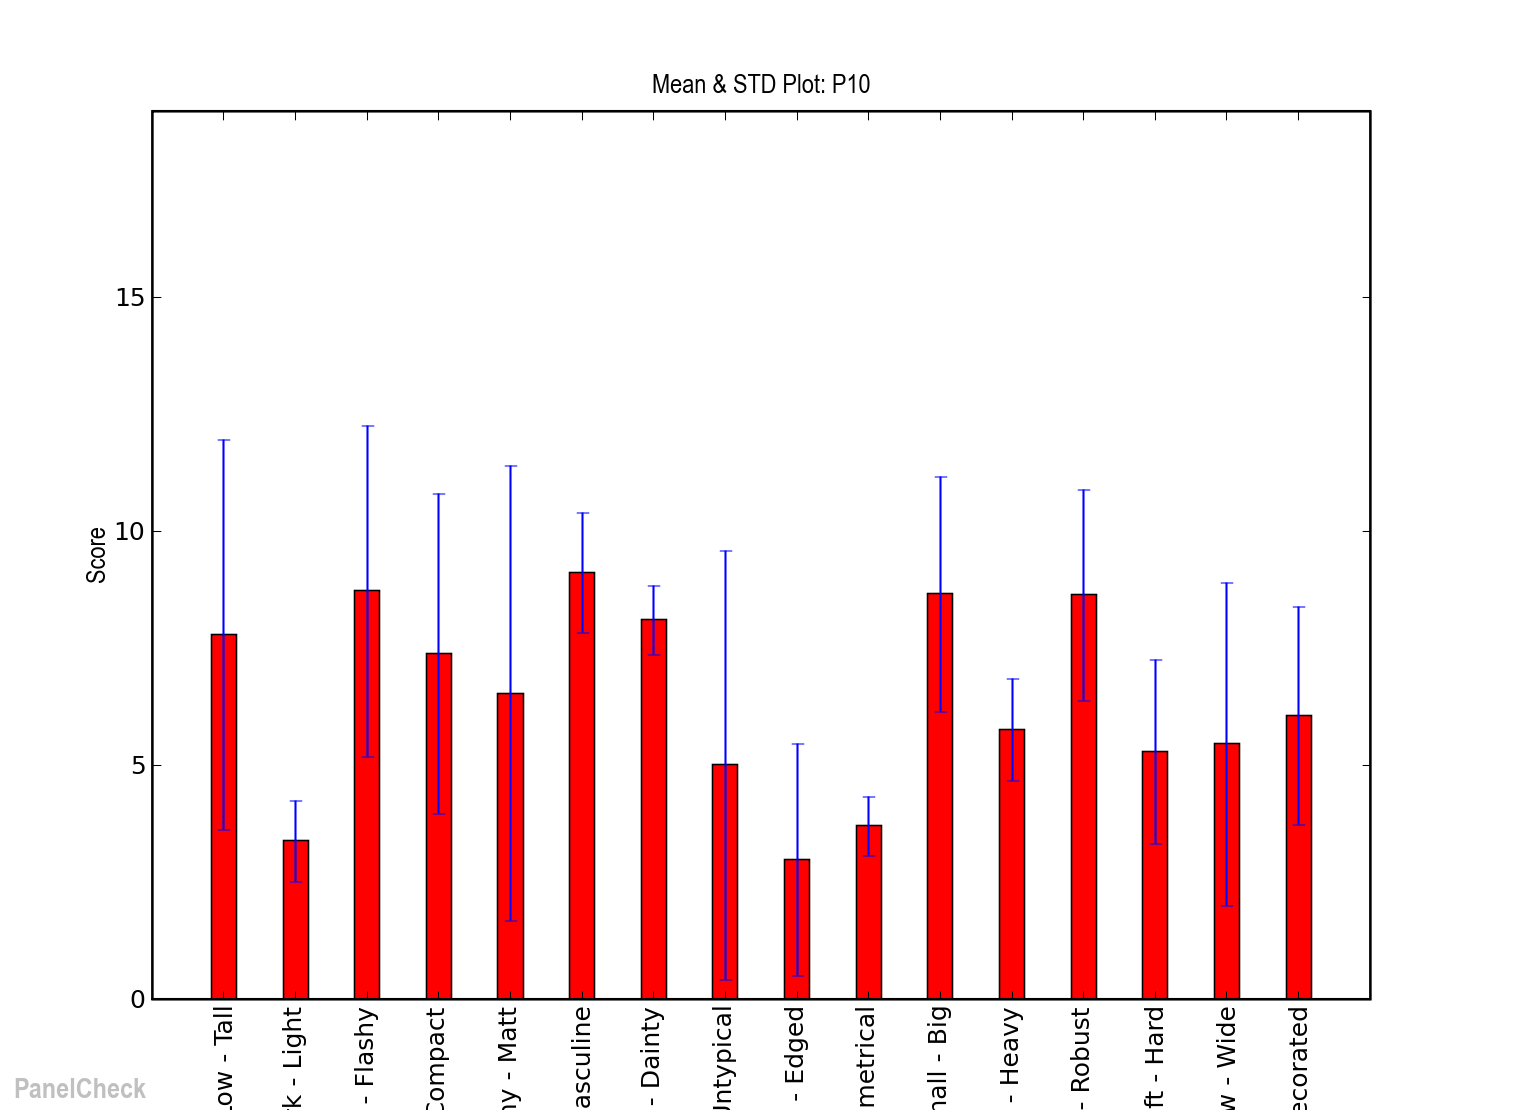
\includegraphics[width = 0.8\textwidth]{Figure/AttributeImportance.png} 
\caption{}
\label{fig:AttributeImportance}
\end{figure}

Looking at the product effect alone for all of the five speakers does not tell us anything about which of the speakers where rated different than the others, but only that some of them were. By doing a 2-way ANOVA on only two of the speakers, it is possible to see which attributes seperates the two. For example, when comparing the Beolab 4000 with the Beolab 6000 (see \autoref{fig:speakers}), the main differentiators are low-tall, light-dark and wide-narrow, as shown in \autoref{fig:4000vs6000}. This approach can be repeated across the different combinations of speakers, to assess how each differs from the others.

\begin{figure}[H]
\centering
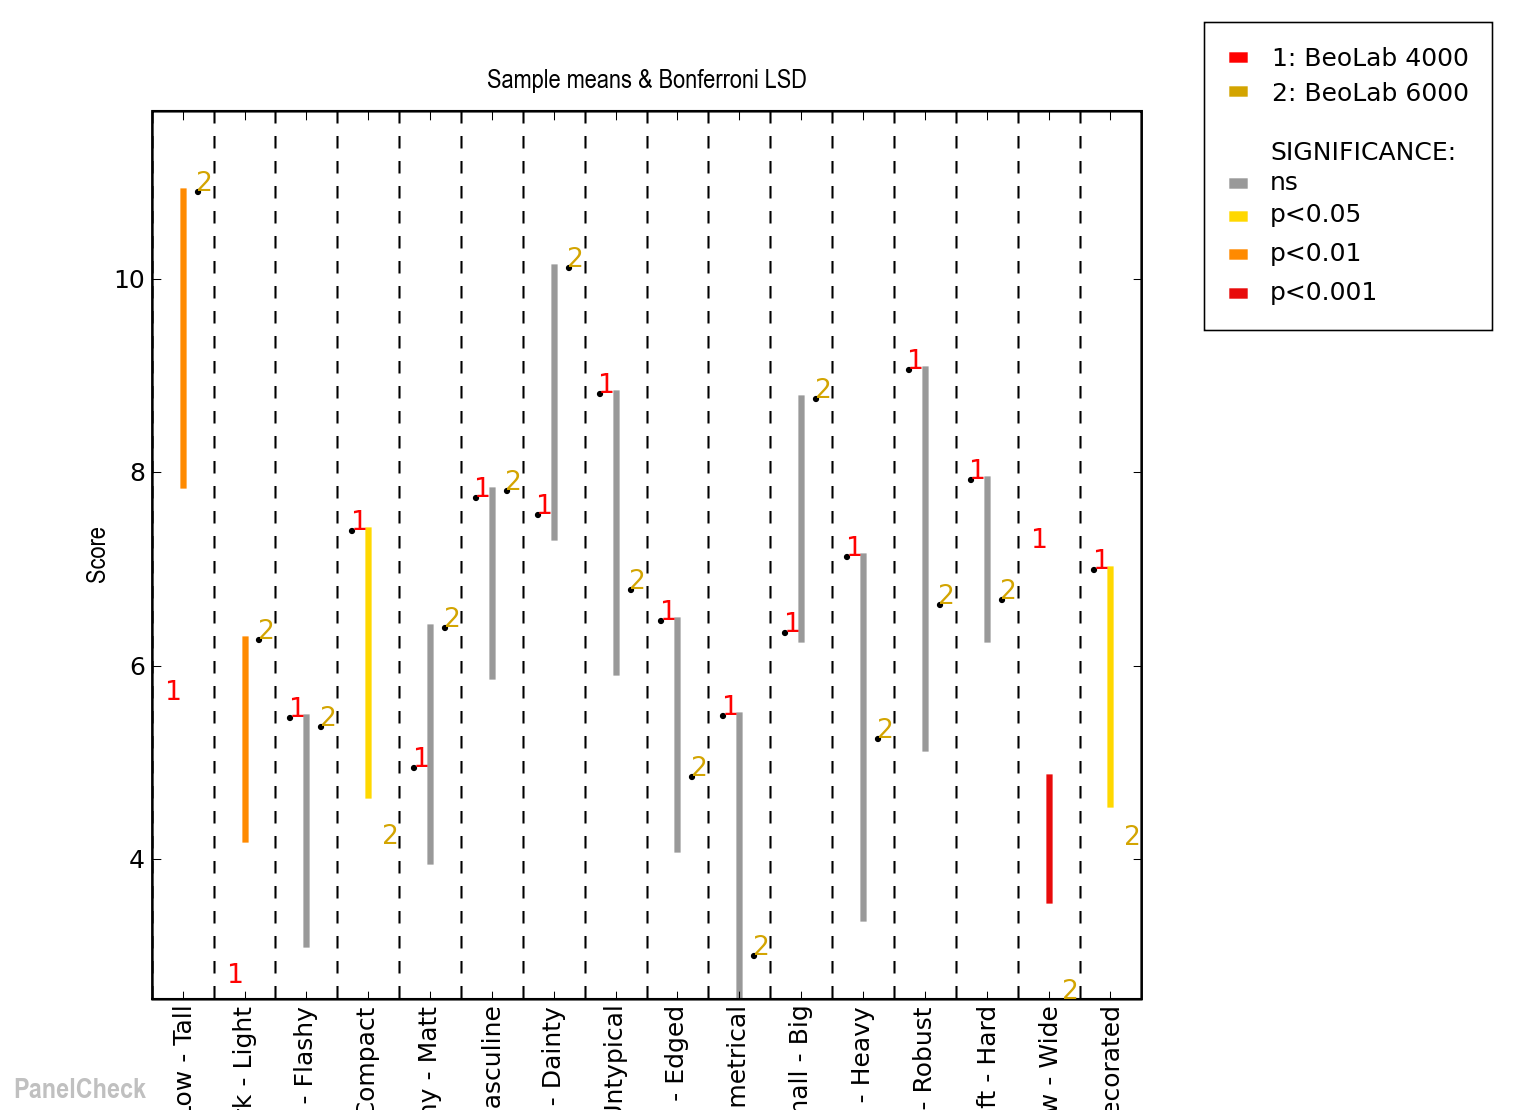
\includegraphics[width = 0.8\textwidth]{Figure/4000vs6000.png} 
\caption{Comparison of the attribute ratings for the Beolab 4000 and the Beolab 6000}
\label{fig:4000vs6000}
\end{figure}



It is possible to look at a spider plot in order to get a sense of how the speakers were rated overall, se \autoref{fig:spider_plot}. For example the BeoLab 5 overall scores the highest in the attributes: \textit{Flashy}, \textit{Decorated}, \textit{Wide}, \textit{Untypical}. This seems reasonable when presented with the speakers next to each other in \autoref{fig:speakers}. In general this paints a fitting picture over which features stands out the most and creates a unique attribute profile for each speaker when shown individually. However when shown all together as in \autoref{fig:spider_plot} a lot of points do end up close to each other and some insights may be lost due to this.

\begin{figure}[H]
\centering
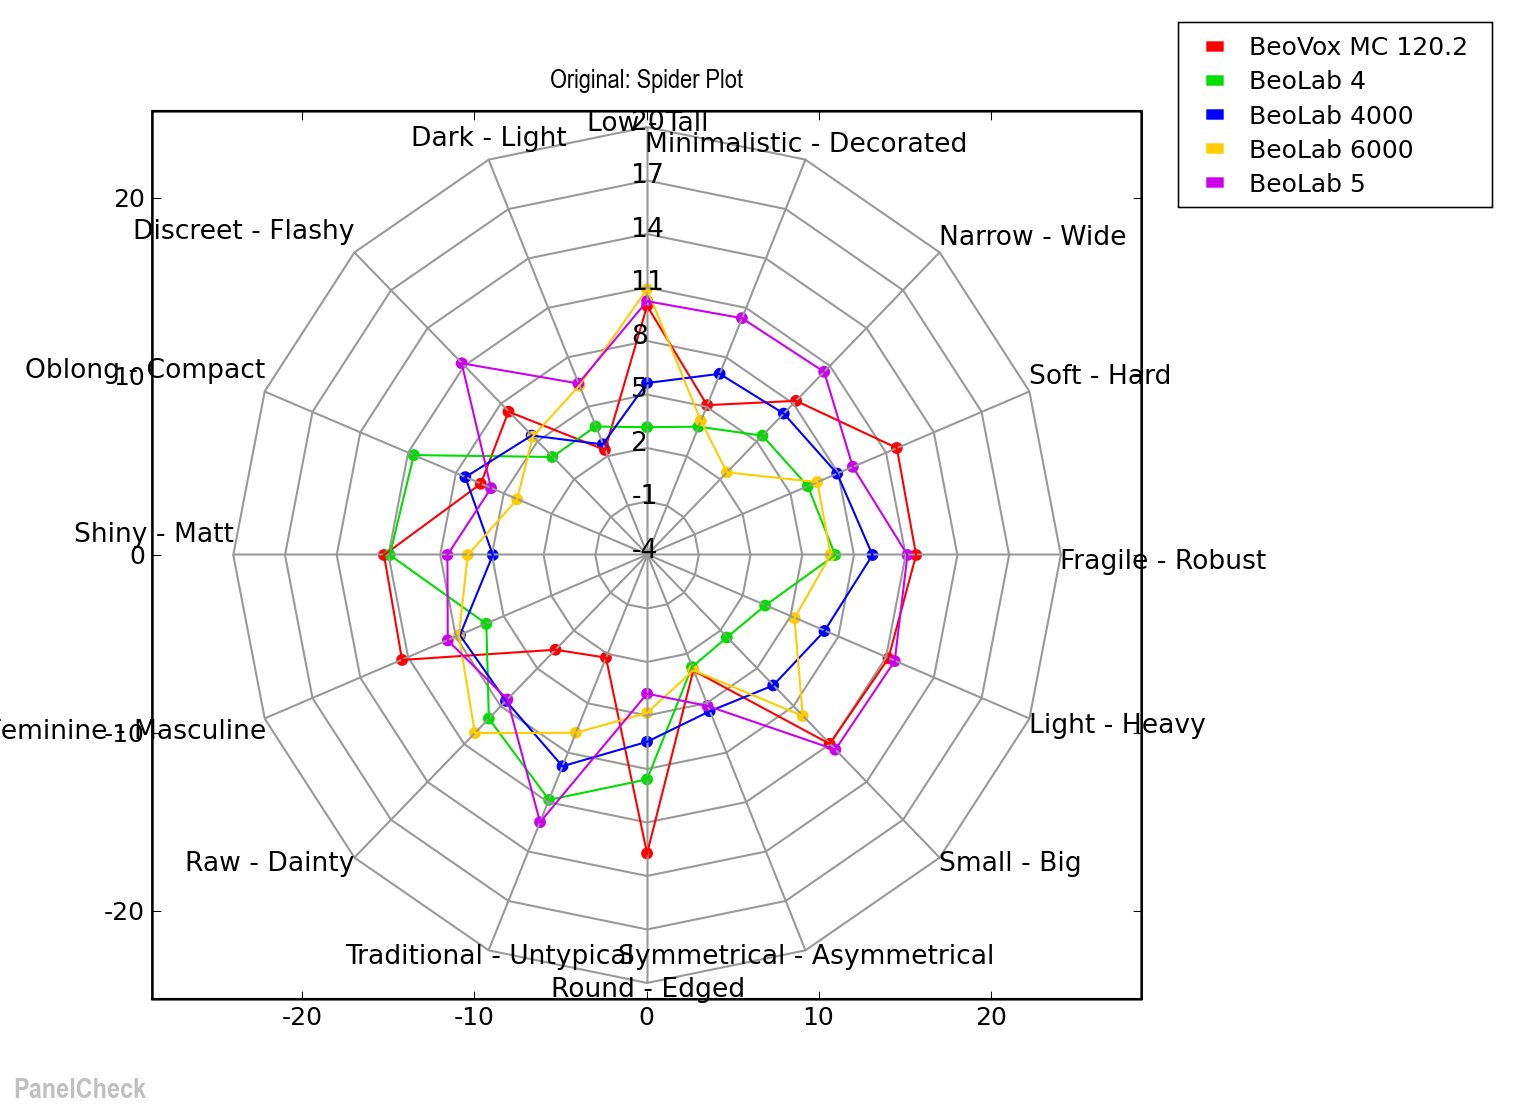
\includegraphics[width = \textwidth]{Figure/spider_plot.png}
\caption{A spider plot of the subjects' preference of the five different speakers}
\label{fig:spider_plot}
\end{figure}